\documentclass[12pt,a4paper]{article}

\usepackage[margin=1in]{geometry}
\usepackage{fancyhdr}
\usepackage{graphicx}
\usepackage{epsfig}
\usepackage{parskip}
\usepackage[ansinew]{inputenc}
\usepackage{amsmath}
\usepackage{amssymb}
\usepackage{bm}
\usepackage{float}
\usepackage[free-standing-units=true]{siunitx} % for consistent handling of SI units
\usepackage[colorlinks=true, pdfstartview=FitV, linkcolor=blue, citecolor=blue, urlcolor=blue]{hyperref} % enable links

\setlength{\parindent}{0pt}

\newcommand{\m}[1]
{\mathrm{#1}}

% Guidelines for reporting
% - pdf
% - scematics
% - Stay scientificly relevant
% - Explain calibration
% - Formula needed


\title{Experiment 83: Do-it-yourself Spectrometer}
\author{Noa Sendlhofer, Christian Leser}
\date{\today}

\begin{document}

\maketitle

\begin{abstract}
    The goal of this experiment series is to determine the temperature of absolute zero, 
    as well as the temperature of liquid nitrogen. An apparatus of constant volume is filled with a gas
    and connected to a pressure sensor. Changing temperatures result in changes in pressure inside the chamber.
    Influences like the pressure and temperature inside the lab, as well as the expansion of the chamber itself
    in changing temperatures must be considered when discussing the obtained data. We concluded that the temperature
    of absolute zero $t_0 = (-275.9 \pm 2.45)\si{\bf\celsius}$ and the temperature of liquid nitrogen $t_{LN2} = (-198.5 \pm 2.56)\si{\bf\celsius}$.
    The literature values lie within our error margins.

\end{abstract}

\tableofcontents

\section{Introduction}

    % Interference double-silt source: https://wiki.anton-paar.com/ch-de/doppelspaltexperiment/
    % Interference grating source: https://www.grund-wissen.de/physik/optik/wellenoptik.html
    % Grating constant source: https://ieeexplore.ieee.org/stamp/stamp.jsp?tp=&arnumber=5547333&tag=1 (eth network)
    % Lands Pits CD source: https://www.researchgate.net/figure/Lands-and-pits-image-using-a-scanning-electron-microscope_fig3_221291847
    

    The goal of this experiment series is to build a spectrometer using household objects by making use of the wave character of light.
    To understand how the spectrometer works, we need to take a close look at how light behaves under certain conditions.

    \begin{figure}[H]
        \centering
        \includegraphics[scale = 0.7]{src/images/interference_double_slit.jpg}
        \caption{Double slit experiment.
        The interference of the light waves produce aspecific pattern which depends of the wavelength of the light entering the slits as well as the distance between the slits. \cite{src_double_slit}}
        \label{fig_double_slit}
    \end{figure}

    Light travels in a spherical way behind a slit meaning that each slit acts as a new source of waves.
    These waves interfere with each other as they overlap, resulting in an interference pattern of alternating bright and dark regions on the screen or detector.
    This behaviour is due to the fact that two maxima or minima intensify each other while a maximum and a minimum cancel out.
    We also refer to these two cases as constructive and destructive.
    Figure~\ref{fig_double_slit} shows how this effect works.

    \begin{minipage}{0.99\linewidth}
        \begin{minipage}{0.7\linewidth}
            \begin{figure}[H]
                \centering
                \includegraphics[scale = 0.25]{src/images/interference_grating.png}
                \caption{A grating leads to a similar effect as a double slit.
                $\Delta s$ is equal to the wavelength.
                As seen in the figure, the angle at which brighter spots of light can be seen depends on the wavelength. \cite{src_grating}}
                \label{fig_grating}
            \end{figure}
        \end{minipage}
        \begin{minipage}{0.25\linewidth}
          \begin{scriptsize}
            \begin{center}
                \begin{figure}[H]
                    \centering
                    \includegraphics[scale = 0.15]{src/images/lands_pits_cd.png}
                    \caption{Lands and pits image of a CD using a scanning electron microscope. These form a grating too. \cite{src_cd}}
                    \label{fig_lands_pits}
                \end{figure}
            \end{center}
            \end{scriptsize}
        \end{minipage}
    \end{minipage}

    Moving on to a grating, it can be abstracted as a lot of slits next to each other.
    Hence, the effect is almost the same as the one observed at the double slit.
    Most importantly, an interference pattern can be observed too.
    When taking a close look at a CD, we notice a grating, presented in figure~\ref{fig_lands_pits}.
    In consequence, a CD must also produce an interference pattern in which light of different wavelength can be observed and distinguished.
    The characterisation of the light is done by measuring the distance of the maximum of first order as it is dependent of the wavelength.

    \begin{minipage}{0.99\linewidth}
        \begin{minipage}{0.45\linewidth}
            \begin{figure}[H]
                \centering
                \includegraphics[scale = 0.4]{src/images/experimental_setup.png}
                \caption{Schematic of the experimental setup.
                A source emits rays of light of which a small portion enters the apparatus through a gap between two razor blades of about 0.2 mm.
                the light then travels through the dark chamber, until it hits the CD.
                After passing through the grid on the CD, an interference pattern can be detected using a camera.}
                \label{fig_setup}
            \end{figure}
        \end{minipage}
        \begin{minipage}{0.1\linewidth}
        \end{minipage}
        \begin{minipage}{0.45\linewidth}
          \begin{scriptsize}
            \begin{center}
                \begin{figure}[H]
                    \centering
                    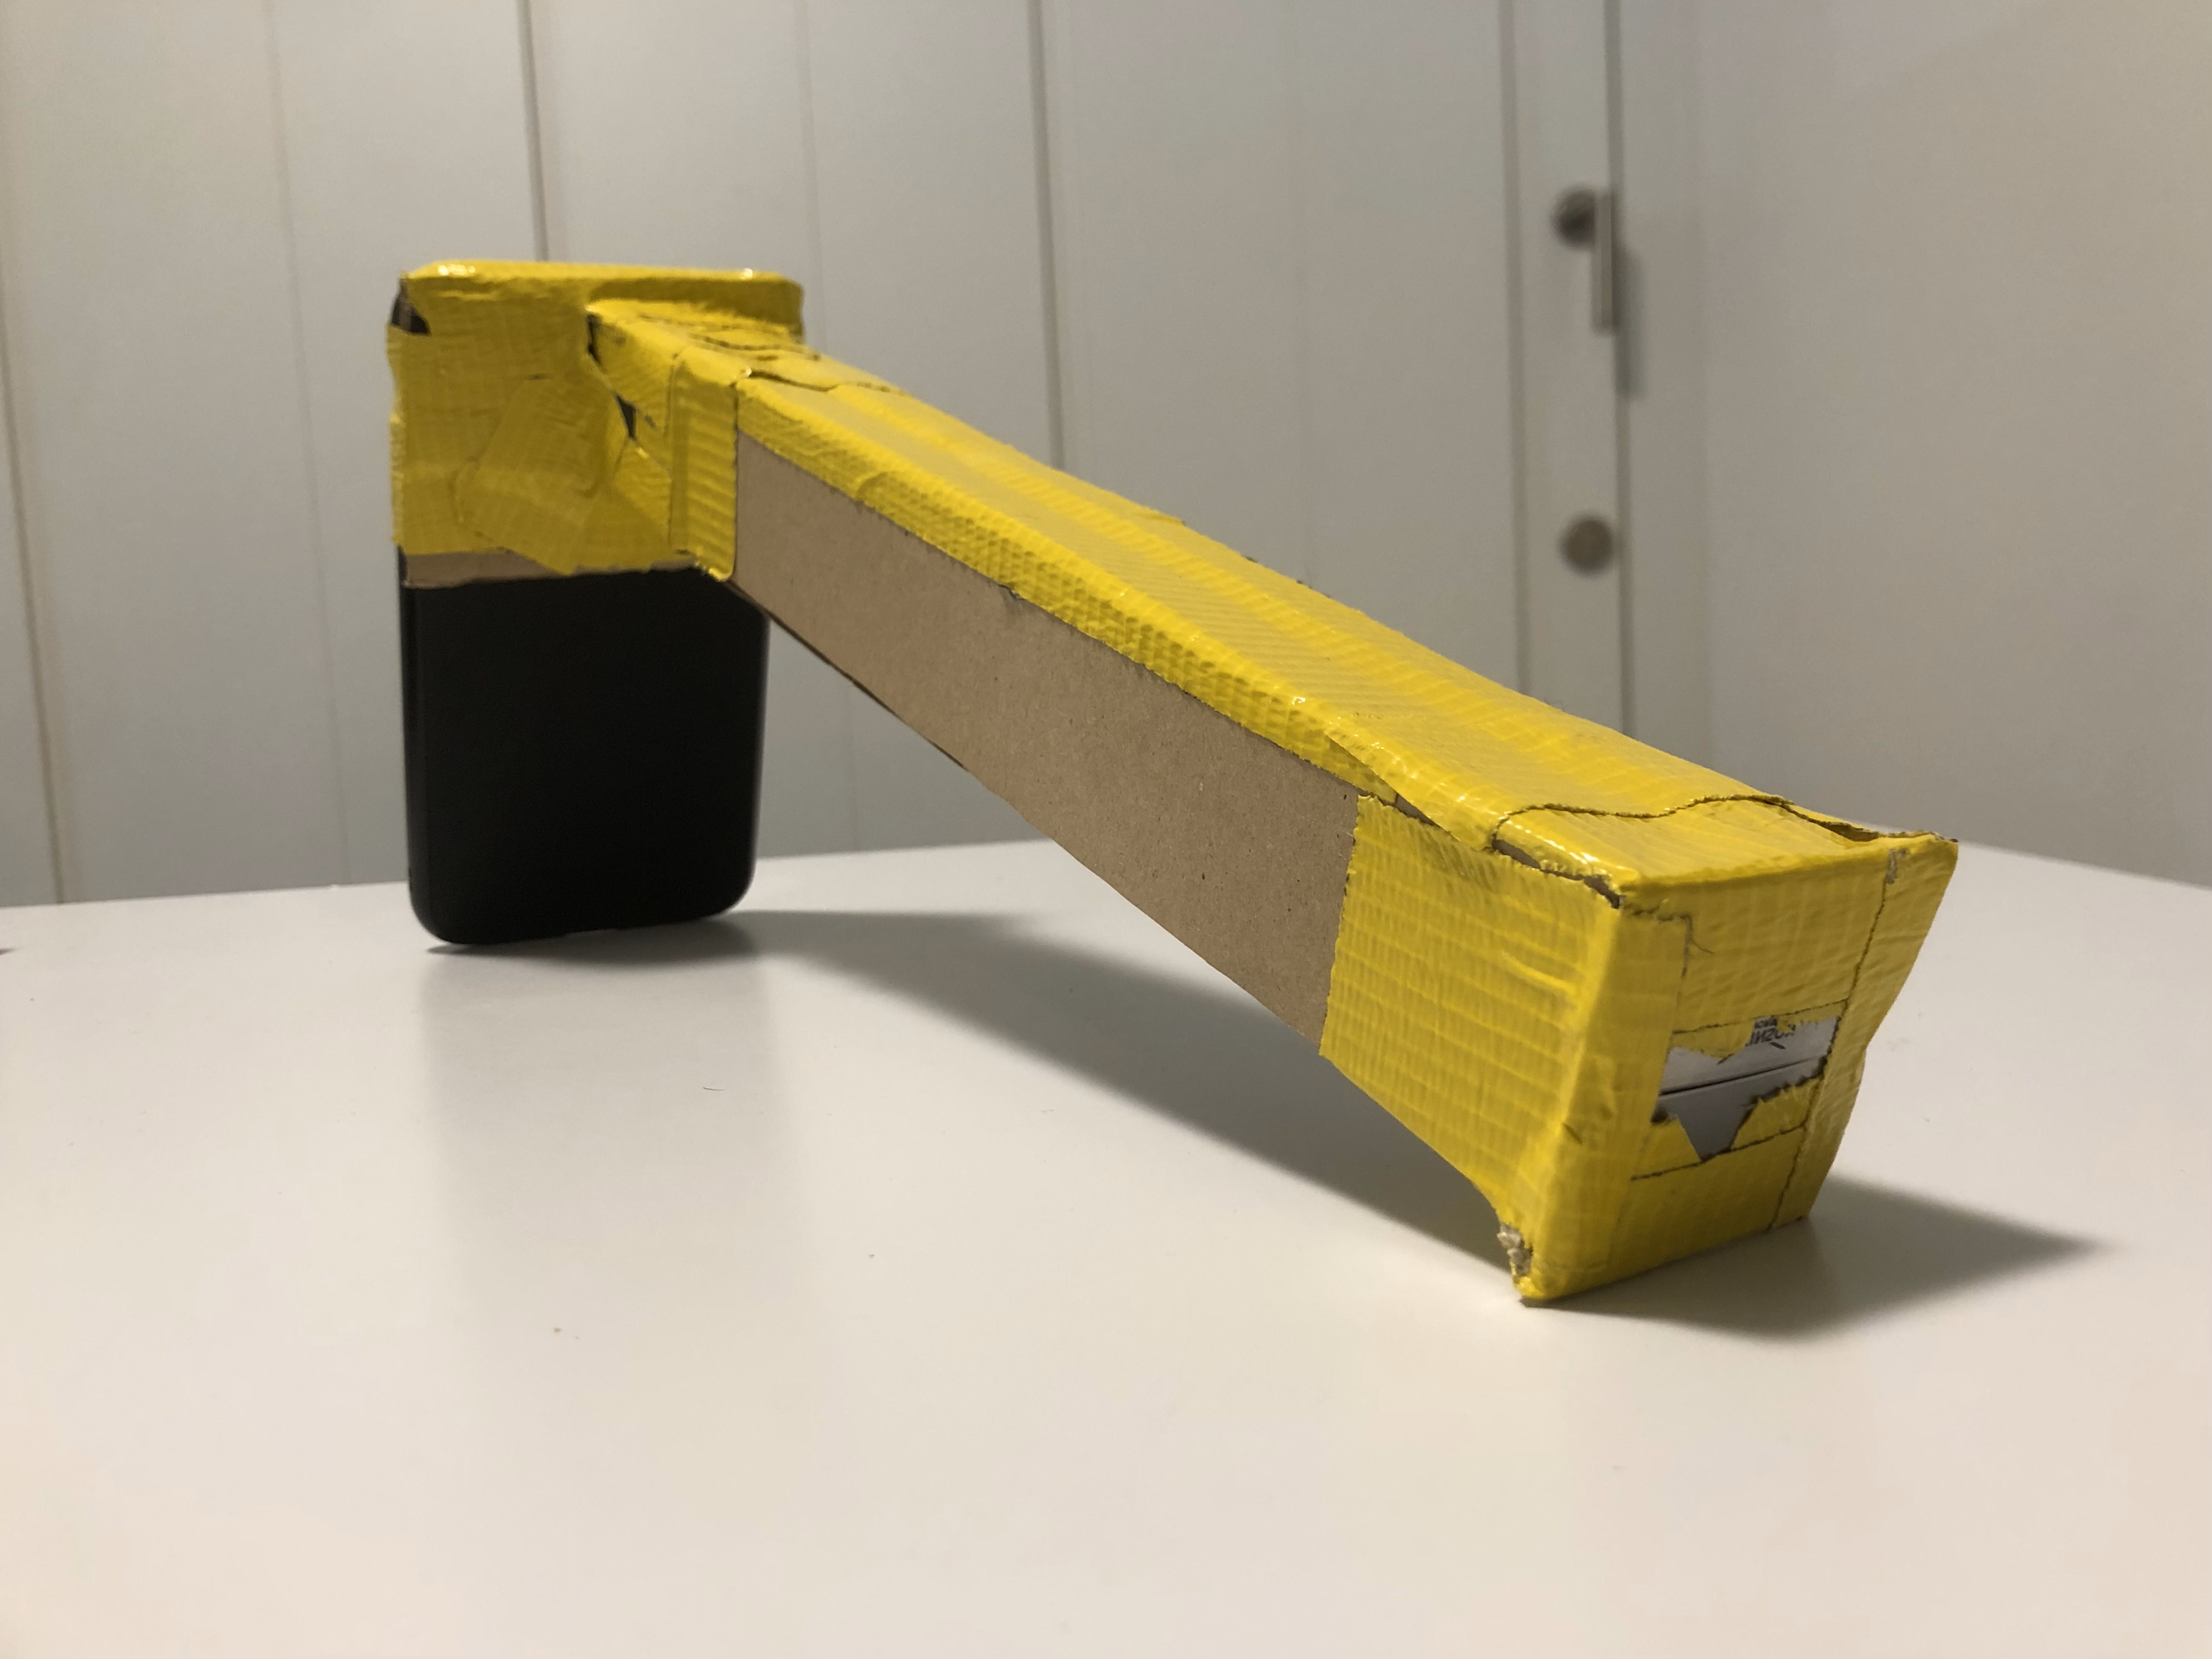
\includegraphics[scale = 0.05]{src/images/spectrometer.png}
                    \caption{Experimental setup used in our case.
                    A phone is used as the camera to detect the interference pattern.}
                    \label{fig_spectrometer}
                \end{figure}
            \end{center}
            \end{scriptsize}
        \end{minipage}
      \end{minipage}
    


    % In general this section should tell the reader why he or she should
    % be interested in your paper. Give some background to the
    % experiment, and describe the underlying principles. This is typically where you provide references to previous publications~\cite{Sato2003}. % Christian

\section{Methodology}
    % Über Bau des Spektrometers erzählen
    % Formeln erklären
    % Argumentieren warum wir grating constant vom internet nehmen

    To build the spectrometer, cardboard, tape, two razor blades, a CD and a camera (ideally wide angle) is needed.
    The less reflective the cardboard is, the better the results are going to be.
    Build a tube with the cardboard and attach the two razor blades to one end, leaving just a small slit of about 0.2 mm for light to enter.
    Remove the reflective foil off the CD using a cutter and tape and cut out a piece of the transparent part of the size of the cardboard tube.
    tape it to the open end of the tube.
    Now attach the camera to the same side.
    make sure no light enters the apparatus except through the slit.

    If held in the direction of a light source, a diffraction pattern, showing the spectrum of the different wavelengths, is visible on the camera.
    The formula relating the distance of the maxima of different orders to the wavelength of the light entering the spectrometer is given in equation~\eqref{eq_interference}.

    \begin{align}
        p \lambda = g \sin(\phi) \label{eq_interference}
    \end{align}

    $p$ is an integer called the order number. For the first visible maximum, $p$ is equal to $1$, for the second maximum $p = 2$ and so on.
    $\lambda$ is the wavelength of the light.
    The grating constant $g$ is dependent on the distance between the slits in the grating.
    Hence this constant is not the same for different kinds of CDs or DVDs.
    the last variable is the angle $\phi$ in the triangle of the maximum of zero and $p^{th}$ order and the spot where the light passes through the grating, measured at the grating.
    Trigonometry gives the relation $\tan(\phi) = \frac{x_p}{d}$, which is visible in the figure~\ref{fig_phi}.

    \begin{figure}[H]
        \centering
        \includegraphics[scale = 0.7]{src/images/angle_phi.png}
        \caption{Visualization of the location of the angle $\phi$ referred to in equation~\eqref{eq_interference}.
        The first and second maximum of one certain wavelength is shown, so monochromatic light would be needed to reproduce this hypothetical situation.}
        \label{fig_phi}
    \end{figure}

    In our test case, we assumed a grating constant $g = 1.514 \mu m$ \cite{src_grating_constant} as we did not have a monochromatic light source at hand to determine the grating constant of our CD.
    Next, we calculated the distance between the CD and the camera to calibrate our spectrometer using a first measurement and by choosing a certain colour and its corresponding wavelength.


    We have multiple goals in this experiment series:
    \begin{enumerate}
        \item The calibration of the pressure sensor and its corresponding pressures.
        \item Determination of the absolute zero point of temperature.
        \item Determination of the temperature of liquid nitrogen.
    \end{enumerate}
    We will achieve these results by making use of the linearly corresponding properties of ideal gases with the help of the apparatus shown in Fig.~\ref{fig_setup}.

    

    Starting with the calibration of the voltmeter, the voltages at room pressure and when a vacuum pump is connected are noted and compared to the actual pressure in the room and the pressure, the pump is able to maintain.
    Hereafter, the glass bulb is evacuated and filled with helium, the reason being that the properties of helium are closer to ideal gases than air.
    Moreover, the oxygen from the air would liquefy when cooled down to the temperature of liquid nitrogen (which would happen in the third step of the experiment series) and liquids do not act according to the ideal gas equation.

    In the next step, the helium-filled glass bulb is heated to the boiling point of water using steam while leaving the apparatus open so that excess helium can escape.
    We chose the temperature of boiling water as the value can easily be calculated using ambient temperature and pressure as well as tabulated data.
    The gas will only expand in this step and hence no air will get into the glass bulb.
    As soon as the helium has reached the desired temperature, the voltage is taken and the system is closed back up at opening 6. (see Fig.~\ref{fig_setup})
    From now on, the closed system can be used just like a thermometer when calculating the temperature at its corresponding voltage.
    
    To create a linear relation of pressure and temperature in the bulb, a second measurement is needed.
    The temperature at the freezing point of water is also known, so this is the second point used in our case.
    The Helium filled bulb is cooled in an ice bath and the voltage is taken.
    To calculate the absolute zero point of temperature, we have to pay respect to the expansion of the glass bulb with increasing temperature.
    Please refer to section~\ref{sec_results} for the calculation.

    As mentioned before, the closed system acts like a thermometer.
    Therefore, we can cool down the helium filled bulb using liquid nitrogen, read off the voltage and calculate the corresponding temperature of liquid nitrogen.
    In this step, the expansion of the glass bulb must be taken into account as well.

    The error sources in this experiment can be classified:
    \begin{itemize}
        \item In our analysis, it is assumed that the temperature in the room stays the same during the whole process.
        Needless to say that this does not have to be the case: small fluctuations happen naturally.
        As a result, corrupted data could occur during the calibration of the sensor.
        Furthermore, the temperature was read off an analog thermometer leading to an uncertainty caused by the limits of the human eye.
        \item Next to the temperature, the pressure does also fluctuate over time.
        The boiling point of water depends on the pressure.
        Hence, when heating the helium to the boiling point of water, a deviation in the temperature used in calculations below and the real temperature could exist.
        As with temperature, the pressure was also read off an analog measurement device and this value could slightly differ from the real pressure.
        \item The manufacturer of the sensor has defined a certain nonlinearity in the conversion of pressure to its corresponding voltage.
        \item The pump does not create an absolute vacuum and small amounts of air could stay in the glass bulb.
        This would have the biggest impact on the temperature measurement of liquid nitrogen as parts of the air would liquify and the linearity resulting from the ideal gas law eq.~\ref{eq_igl} would not be maintained.
        \item When heating and cooling the gas in the bulb, the glass itself could need more time to evenly distribute the temperature resulting in an uneven change in the gas volume, therefore changing the pressure.
        This would affect the difference between the linear approach and the exact calculation of $t_0$ and $t_{LN2}$.
    \end{itemize}
 % Christian

\section{Results}\label{sec_results}

In our case, we will calculate the grating constant $g$ using hypothetical values for the reasons mentioned in section \textbf{insert section and information from GPT}
By rearranging and combining eq.\ref{eq_interference} and eq.\ref{eq_phi} we find a formula for the grating constant\ref{eq_g}.

\begin{align}
    g &= \frac{p \lambda}{\sin(\phi)} \label{eq_g}\\
    \phi &= \arctan \left( \frac{x}{D} \right)
\end{align}

To calculate the uncertainty of the grating constant, the gaussian error propagation is a useful tool.

\begin{align}
    \Delta g &= \sqrt{\left( \frac{\partial g}{\partial p} \Delta p \right)^2 + \left( \frac{\partial g}{\partial \lambda} \Delta \lambda \right)^2 + \left( \frac{\partial g}{\partial \phi} \Delta \phi \right)^2}\\
    \Delta \phi &= \sqrt{\left( \frac{\partial \phi}{\partial x} \Delta x \right)^2 + \left( \frac{\partial \phi}{\partial D} \Delta D \right)^2}
\end{align}

The hypothetical value of the grating constant $g$ and its uncertainty can now be calculated:

\begin{align}
    \bf g = (1520 \pm 20) ~\si{\bf\nano\meter} = (1.52 \pm 0.02) ~\si{\bf\micro\meter} \label{res_g}
\end{align}

Note that the obtained value is not the real value and that a different value for the grating constant $g$ \cite{src_grating_constant} is used in the remaining calculations.

As mentioned in the previous chapter, the first goal is to find the distance $d$ of the grating
and the image sensor.
By combining eq. \ref{eq_interference} and eq. \ref{eq_phi} we get the following equation for $d$:

\begin{align}
    d = \frac{x}{\tan(\phi)} = \frac{x}{\tan(\arcsin(\frac{\lambda}{g}))} \label{eq_distance}
\end{align}

Multiple steps are necessary to calculate the distance $d$.
First of all, we took a picture with the spectrometer pointed at the sunlight \ref{fig_sunlight}. We then selected suitable 
points in the spectrum and compared them to tabulated wavelengths and their corresponding colors 
in fig.~\ref{fig_wavelengths}. In the next step we measured the distance of said points to the zero-order maximum
using the imtools method in matlab. This is our pixel distance $x$ in eq.~\ref{eq_distance}.

For our final calculation of the distance $d$ we averaged multiple measurement points to get a more
accurate result. This is shown in fig.~\ref{fig_distance_calc}.

The error calculations for eq. \ref{eq_distance} were done using the gaussian error propagation.
Please refer to our jupyter notebook \cite{GitHub}, for the full calculations of all the values and 
error propagations presented in this chapter. 
\begin{align}
    \Delta d = \sqrt{\left(\frac{\partial d}{\partial x}\right)^2 + \left(\frac{\partial d}{\partial \lambda}\right)^2}
\end{align}

Our averaged result for $d$ is:
\begin{align}
    \bf d = (1.71 \pm 0.12) ~\si{\bf\milli\meter} \label{res_d}
\end{align}

We have now successfully calibrated our spectrometer and we can now determine the wavelength
of any point in the picture.
The following equation is used to determine the wavelength of a point with a certain pixel 
distance $x$ to the zero-order maximum.
\begin{align}
    \lambda = g \sin\left(\arctan\left(\frac{x}{d}\right)\right) \label{eq_lambda}
\end{align}

Again the uncertainties were determined using the gaussian error propagation.
\begin{align}
    \Delta \lambda = \sqrt{\left(\frac{\partial \lambda}{\partial x}\right)^2 + \left(\frac{\partial \lambda}{\partial d}\right)^2}
\end{align}

Using these obtained results we finally analyzed some different types of light
sources. In each case, we assumed an error of $\pm 10$ pixels, since we had to guess the position of each measurement point in the picture.

\newpage

First of all, we analyzed a fluorescent tube lamp. As can be seen in fig. \ref{fig_lamp1} below, this type of light source only emits certain small 
ranges of wavelength. In our case, we measured the following ranges:
\begin{alignat}{3}
    &\text{Red spectrum:} \; &&(587 \pm 36)~\si{\nano\meter} & &- (622 \pm 38)~\si{\nano\meter} \nonumber\\
    &\text{Green spectrum:} \; &&(487 \pm 32)~\si{\nano\meter} & &- (560 \pm 35)~\si{\nano\meter} \nonumber\\
    &\text{Blue spectrum:} \; &&(430 \pm 29)~\si{\nano\meter} & &- (455 \pm 31)~\si{\nano\meter} \nonumber
\end{alignat}
\begin{figure}[H]
    \centering
    \includegraphics[scale = 0.31]{src/images/lamp1_meas.png}
    \caption{Spectrum of a fluorescent tube.}
    \label{fig_lamp1}
\end{figure}

As a second example, we analyzed a LED ceiling lamp. As can be seen in fig. \ref{fig_lamp2} below, this lamp
emits almost the entire spectrum of visible light with no gaps visible. We measured the following range:
\begin{alignat}{3}
    &\text{Full spectrum:} \; &&(429 \pm 29)~\si{\nano\meter} & &- (650 \pm 38)~\si{\nano\meter} \nonumber
\end{alignat}
\begin{figure}[H]
    \centering
    \includegraphics[scale = 0.41]{src/images/lamp2_meas.png}
    \caption{Spectrum of an LED ceiling light.}
    \label{fig_lamp2}
\end{figure}

Lastly, we analyzed the computer screen of a laptop. In this example, the color purple was shown on the screen.
As can be seen in fig. \ref{fig_purple_screen} only two very narrow bands of wavelengths are emitted.
\begin{alignat}{3}
    &\text{Red spectrum:} \; &&(597 \pm 37)~\si{\nano\meter} & &- (622 \pm 38)~\si{\nano\meter} \nonumber\\
    &\text{Blue spectrum:} \; &&(433 \pm 29)~\si{\nano\meter} & &- (457 \pm 37)~\si{\nano\meter} \nonumber
\end{alignat}
\begin{figure}[H]
    \centering
    \includegraphics[scale = 0.25]{src/images/purple_screen_meas.png}
    \caption{Spectrum of a computer screen displaying a purple color.}
    \label{fig_purple_screen}
\end{figure}

Helium discharge tube
Quecksilver light, UV A 400nm, UV C 250nm % Noa

\section{Conclusion}
    In this experiment, we successfully built a spectrometer using the grating feature of a cd.
    As a first step, we were required to calibrate the spectrometer.
    As we did not have a monochromatic light source at hand, we used a literature value for the grating
    constant $g$. Next, we had to determine the distance $d$ of the camera sensor and the grating.
    We concluded that $\bf d = (1.7 \pm 0.1) ~\si{\bf\milli\meter}$.
    Finally, we were able to analyze some different light sources, to determine their respective wave spectrums.
    We found that some indoor ceiling lights emit only certain wavelengths, while others emit almost the entire
    visible spectrum.
    We are very happy with how our spectrometer turned out. We can calculate the wavelength of any color
    in the detected spectrum, with a satisfactory error margin.

    Unfortunately, we were not able to detect Frauenhofer lines in our measurements taken from sunlight.
    This is due to the fact, that our device is not accurate enough to distinguish these fine lines in the spectrum.
    To improve this result, we would have to make the following changes to our device:
    \begin{itemize}
        \item Improve the consistency in the gap of the razor blades.
        \item Coat the inside of the box with a non-reflective dark paint.
        \item Use a higher-resolution camera, with a manual focus setting.
        \item Build a spectrometer using a grating with a smaller grating constant $g$, as this would lead to the same spectrum split into a bigger area.
            A DVD perhaps even with blu-ray-technology could maybe do the job.
    \end{itemize}

    % In the concluding paragraph you summarize the result, with the
    % emphasis on what you have discovered in this work. You can end this
    % with an outlook on future research, i.e. how could the results be
    % improved or what would be a logical follow-up experiment.

\section{Appendix}
        
    \begin{figure}[H]
        \centering
        \includegraphics[scale = 0.25]{src/images/wavelengths.png}
        \caption{Wavelength (nm) and corresponding colors. Also shown are the Frauenhofer lines for the sun's spectrum.}
        \label{fig_wavelengths}
    \end{figure}

    \begin{figure}[H]
        \centering
        \includegraphics[scale = 0.4]{src/images/distance_calc.png}
        \caption{Spectrum of sunlight with measurements taken of certain points.}
        \label{fig_distance_calc}
    \end{figure}


\begin{thebibliography}{99}

\bibitem{src_double_slit}
Anton Paar, Double slit experiment, \href{https://wiki.anton-paar.com/ch-de/doppelspaltexperiment/}{website} (last visited: 2023.05.22)

\bibitem{src_grating}
Grund-Wissen, Lichtbeugung und Interferenz, \href{https://www.grund-wissen.de/physik/optik/wellenoptik.html}{website} (last visited: 2023.05.22)

\bibitem{src_cd}
G. Hammouri, A. Dana, and B. Sunar, CDs Have Fingerprints Too (2014), \href{https://www.researchgate.net/figure/Lands-and-pits-image-using-a-scanning-electron-microscope_fig3_221291847}{website} (last visited: 2023.05.22)

\bibitem{src_grating_constant}
B. Gyoch, T. Pencheva, P. Mashkov, Optical Measurements upon Compact Discs in Education in Optoelectronics, \href{https://ieeexplore.ieee.org/stamp/stamp.jsp?tp=&arnumber=5547333&tag=1}{website} (last visited: 2023.05.23)

\bibitem{GitHub}
GitHub Repository containing calculations and further images. \href{https://github.com/Noothless/Physik-Absolute-Zero}{website}

% How does the light of a computer screen work? https://www.quora.com/What-happens-if-I-shine-a-mixture-of-red-and-green-light-which-makes-yellow-through-a-perfect-yellow-filter

\end{thebibliography}

\end{document}